\section{V5}
\subsection{Data Alignment}
\begin{tabular}{|l|l|l|}
    \hline 
    1 Byte & 8 Bit  & Byte  \\ 
    \hline 
    2 Byte & 16 Bit & Half-Word \\ 
    \hline 
    4 Byte & 32 Bit & Word \\ 
    \hline 
    8 Byte & 64 Bit & Double-Word \\ 
    \hline 
\end{tabular} 

\subsubsection{Aligned-Unaligned Data}
\begin{multicols}{2}
    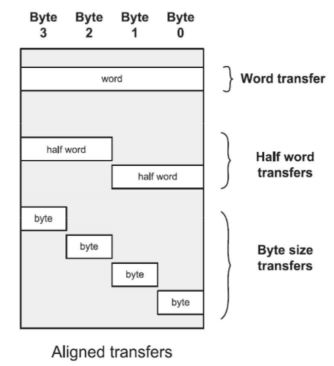
\includegraphics[width=0.5\textwidth]{images/alignedData}
    
    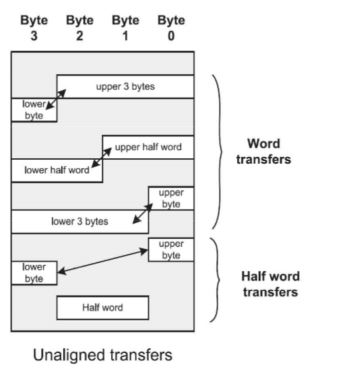
\includegraphics[width=0.5\textwidth]{images/unalignedData}
\end{multicols}
    \clearpage
\subsubsection{Bit-Banding}
\[\textbf{ BitBandAliasAddress = BitBandAliasBase + (MemoryAddres - BitbandRegionBase)* 32 + 4*BitNumber} \]
    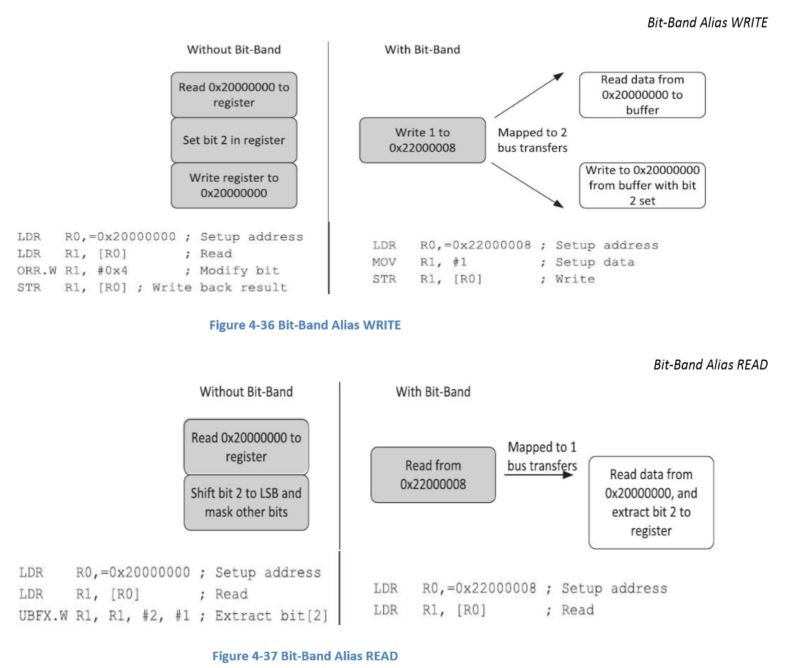
\includegraphics[width=\textwidth]{images/bitbanding}